\chapter{ТЕОРЕТИЧНІ ОСНОВИ КРИПТОСИСТЕМИ НА ОСНОВІ КІЛЕЦЬ}\label{ch:-2:------}

Даний розділ присвячено теоретичному підґрунтю симетричної криптосистеми, запропонованої у цій роботі.
Виходячи з базових понять криптографії та теорії кілець, розглянутих у Розділі~\ref{ch:-1:---}, основна увага приділяється конкретним алгебраїчним структурам і операціям, що використовуються у протоколі.
Аналізуються властивості скінченних кілець $Z_k$ та їх ізоморфних аналогів $G_k$, ключова роль різних відображень (ізоморфізмів, сюр'єкцій, бієкцій) між цими кільцями, а також теорія систем лінійних рівнянь (СЛР) над $Z_m$.
Особливу увагу приділено механізму шифрування, що ґрунтується на перетвореннях та обчисленнях СЛР.
Описано генерацію компонентів системи та теоретичні засади її стійкості.
Розділ зосереджено на розгляді складових механізмів, що готують підґрунтя для повного опису протоколу у Розділі~\ref{ch:-3:---}.

\section{Алгебраїчні структури: скінченні кільця та відображення}
\label{sec:algebraic_structures}
Криптографічний протокол, розглянутий у цій роботі, базується на алгебраїчних властивостях скінченних асоціативно-комутативних кілець з одиницею та спеціальних відображеннях між ними.
Розуміння цих компонентів, спираючись на означення та властивості, наведені у~\ref{sec:ring_theory}, є необхідною передумовою для аналізу механізмів і стійкості системи~\cite{Shoup08, KatzLindell14}.
Далі деталізуються кільця та відображення, що є центральними для протоколу.

\subsection{Скінченні комутативні кільця з одиницею}
\label{subsec:finite_rings}
Основною алгебраїчною структурою є кільце лишків за модулем $k$, позначене $Z_k$, формальне означення та базові властивості якого наведено у~\ref{subsec:residue_rings}.
$Z_k = \{\bar{0}, \bar{1}, \ldots, \overline{k-1}\}$ утворює кільце відносно додавання та множення за модулем $k$.
Ця структура є асоціативною та комутативною, містить адитивну ($\bar{0}$) та мультиплікативну ($\bar{1}$) одиниці, а кожен елемент має адитивний обернений.
Характеристика кільця $Z_k$ дорівнює $k$.

У $Z_k$ особливе значення мають дільники одиниці (елементи з мультиплікативними оберненими, тобто $\gcd(a, k) = 1$) та дільники нуля (ненульові елементи, добуток яких дорівнює нулю).
Дільники одиниці утворюють мультиплікативну групу $Z_k^*$ (див.~\ref{subsec:ring_units_group}).
Дільники нуля існують, якщо $k$ складене, що суттєво відрізняє кільце від поля.

Окрім стандартного представлення $Z_k$, у криптосистемі використовуються кільця $G_k$, які є ізоморфними $Z_k$ (див.~\ref{subsec:ring_mappings}).
$G_k$ будується як скінченне асоціативно-комутативне кільце з одиницею, ізоморфне до $Z_k$, але з іншим конкретним представленням елементів та операцій.
Це досягається спеціальною процедурою побудови, описаною у~\ref{subsec:gen_g_algorithm}, що ґрунтується на визначальному рядку.
Визначальний рядок задає перестановку або перенумерацію елементів $\{0, 1, \ldots, k-1\}$.
Використання $G_k$ замість стандартного $Z_k$ є основним засобом обфускації, що приховує структуру модульної арифметики від стороннього спостерігача, який не знає визначального рядка.
Вибір $G_k$ визначається секретними параметрами, якими обмінюються абоненти.

\subsection{Ізоморфізми кілець (\(\varphi\))}
\label{subsec:ring_isomorphism}
Ізоморфізми кілець, формальне означення яких наведено у~\ref{subsec:ring_mappings}, встановлюють структурну еквівалентність між $Z_k$ та $G_k$.
Протокол використовує ізоморфізм $\varphi: Z_m \to G_m$ (або аналогічний $\varphi_k: Z_k \to G_k$).
Ізоморфізм $\varphi$ є не лише теоретичним об'єктом, а й ключовим механізмом для практичних обчислень.

Наявність $\varphi$ дозволяє виконувати всі необхідні арифметичні операції (додавання, множення, матричні операції) у стандартному кільці $Z_m$.
Для будь-яких $x, y \in G_m$ їх сума або добуток у $G_m$ обчислюється шляхом відображення у $Z_m$ через $\varphi^{-1}$, виконання стандартної операції у $Z_m$, а потім повернення у $G_m$ через $\varphi$:
\begin{gather*}
    x +_G y = \varphi(\varphi^{-1}(x) +_{Z_m} \varphi^{-1}(y))\\
    x \cdot_G y = \varphi(\varphi^{-1}(x) \cdot_{Z_m} \varphi^{-1}(y))
\end{gather*}
Це дозволяє уникнути побудови та зберігання великих таблиць операцій для $G_m$, особливо при великих $m$.

Конкретний ізоморфізм $\varphi$ визначається визначальним рядком, згенерованим для $G_m$ алгоритмом GEN-G (див.~\ref{subsec:gen_g_algorithm}) на основі спільних секретних параметрів.
Наприклад, визначальний рядок $b=(1, 5, 4, 2, 3, 0)$ для $k=6$ задає ізоморфізм $g: Z_6 \to G_6$, де $g(\bar{1})=1, g(\bar{2})=5, g(\bar{3})=4, g(\bar{4})=2, g(\bar{5})=3, g(\bar{0})=0$.
Використовуючи цей $g$, обчислення $5 \cdot 4$ у $G_6$ зводиться до $g(g^{-1}(5) \cdot g^{-1}(4)) = g(\bar{2} \cdot \bar{3}) = g(\bar{0}) = 0$.
Знання цього відображення $\varphi$ (або визначального рядка) є частиною секретного ключа.

На рисунку~\ref{fig:gk_zk_iso} показано візуалізацію ізоморфізму між $Z_k$ та $G_k$.
\begin{figure}[ht]
    \centering
    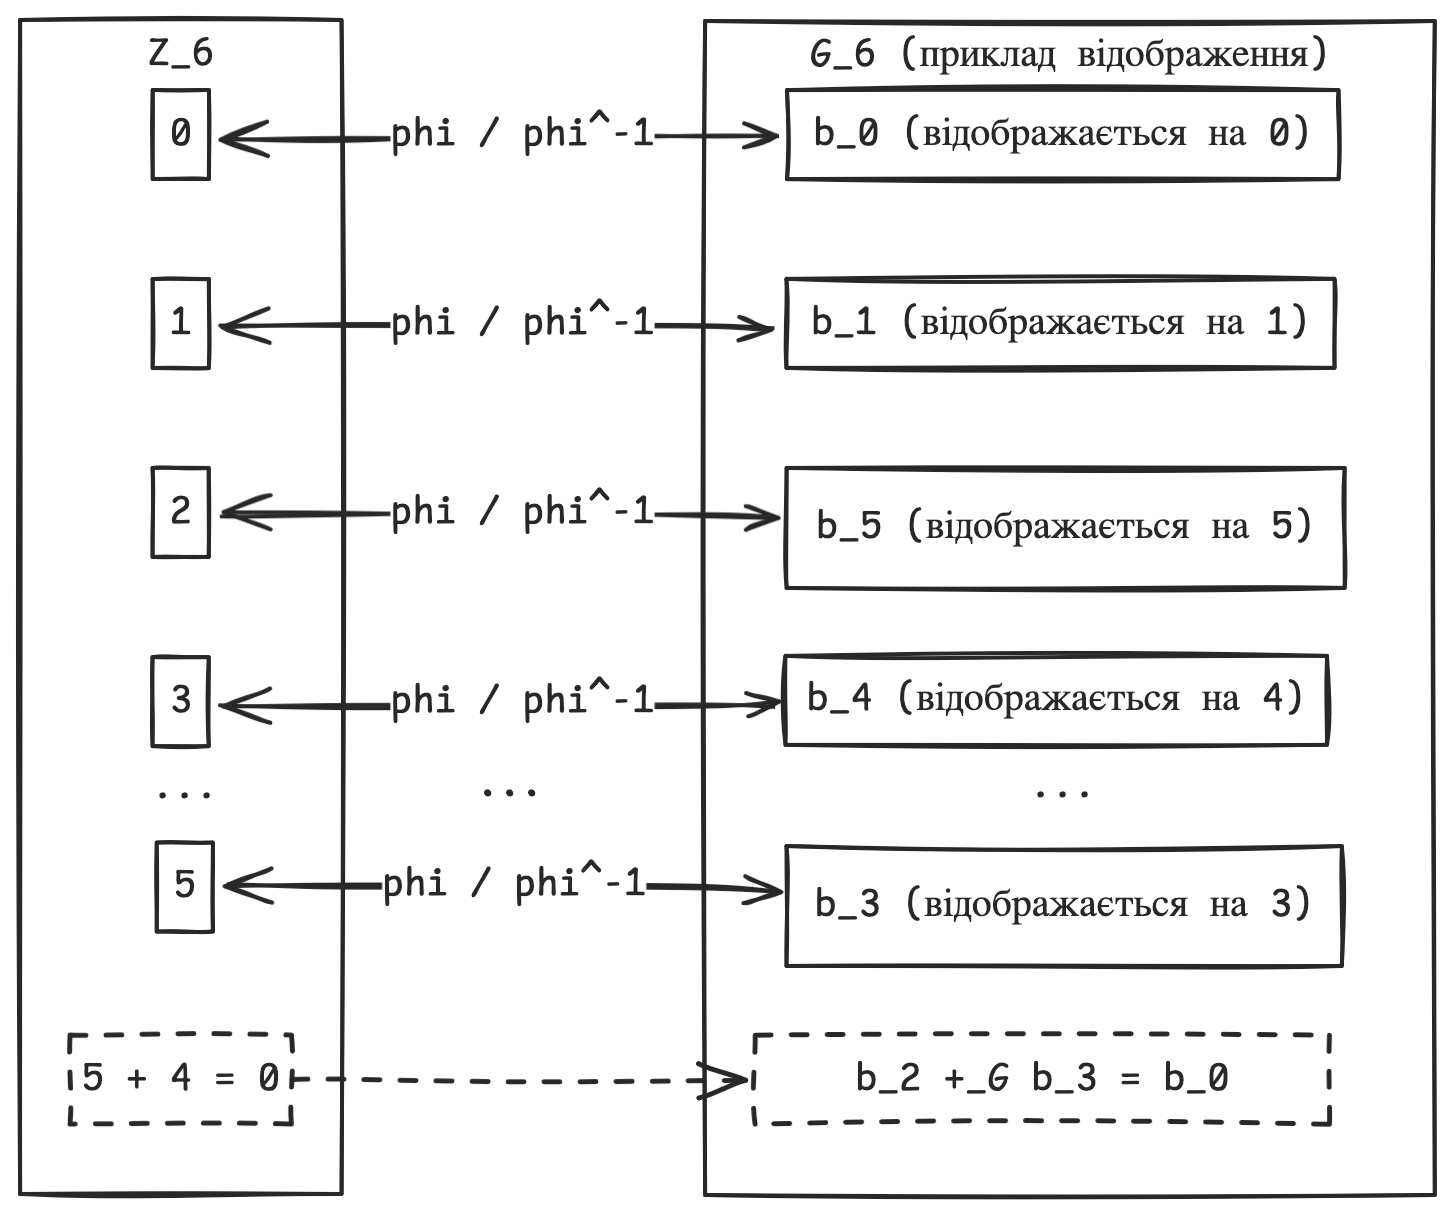
\includegraphics[width=0.5\textwidth]{pictures/G_k vs Z_k Isomorphism Example}
    \caption{Візуалізація ізоморфізму $\varphi$ між $Z_k$ та $G_k$ та відповідності операцій.}
    \label{fig:gk_zk_iso}
\end{figure}

\subsection{Сюр'єкції кілець ($\psi, \lambda$) та фактор-множини}
\label{subsec:ring_surjection}
Окрім ізоморфізмів, протокол використовує сюр'єктивні гомоморфізми (сюр'єкції), означення яких наведено у~\ref{subsec:ring_mappings}.
Ці відображення проектують інформацію з більшого кільця $G_k$ на менше робоче кільце $G_m$.
Архітектура протоколу (див. рис.~\ref{fig:schema}) містить дві такі сюр'єкції: $\psi: G_k \to G_m$ та $\lambda: G_k \to G_m$.
Для їх природного означення $k$ зазвичай вибирається кратним $m$, тобто $k=lm$.
Типовим прикладом є природне відображення $\pi: Z_k \to Z_m$, де $\pi(\bar{a} \bmod k) = \overline{a \bmod m}$, що є гомоморфізмом кілець при $m|k$.

Кожній сюр'єкції $\psi: G_k \to G_m$ відповідає її ядро $\ker \psi = \{x \in G_k \mid \psi(x) = 0_G\}$, яке є ідеалом у $G_k$.
Фактор-множина $G_k/\psi$ (точніше, фактор-кільце $G_k/\ker \psi$) складається з класів суміжності ядра, тобто множин вигляду $x + \ker \psi = \{x+y \mid y \in \ker \psi\}$ для $x \in G_k$.
Як зазначено у~\ref{subsec:factor_rings}, перша теорема про ізоморфізм гарантує, що $G_k/\ker \psi \cong \mathrm{Im}(\psi)$.
Оскільки $\psi$ сюр'єктивне на $G_m$, маємо $G_k/\ker \psi \cong G_m$.

Протокол використовує фактор-множини $G_k/\psi$ та $G_k/\lambda$ як множини прообразів.
Кожному елементу $y \in G_m$ відповідає унікальний клас (елемент фактор-множини), тобто множина $\psi^{-1}(y) = \{x \in G_k \mid \psi(x) = y\}$.
Далі вводяться бієкції $\psi_1: G_k/\psi \to G_m$ та $\lambda_1: G_k/\lambda \to G_m$, які формалізують зв'язок між класами фактор-множини та елементами цільового кільця $G_m$.
Їхня роль полягає в обфускації: значення $y \in G_m$ (або його еквівалент у $Z_m$) публічно представляється не самим $y$, а вибором елемента $x$ з більшого кільця $G_k$, що належить до відповідного класу прообразу ($\psi(x) = y$).
Наприклад, коли Аліса публікує коефіцієнти системи або Боб передає компоненти шифрограми, значення, обчислені у $G_m$ (або $Z_m$), відображаються через $\psi_1$ чи $\lambda_1$ для ідентифікації відповідного класу у $G_k/\psi$ чи $G_k/\lambda$, а потім з цього класу вибирається представник для передачі.
Це приховує справжнє значення $y$ серед великої множини елементів $G_k$, що суттєво ускладнює аналіз для атакуючого, який не знає конкретних сюр\'єкцій $\psi, \lambda$ та бієкцій $\psi_1, \lambda_1$.
Вибір представника у класі може здійснюватися за певним правилом або випадково, що потенційно підвищує стійкість системи.

На рисунку~\ref{fig:obfuscation_flow} показано приклад потоку даних для обфускації та де-обфускації значень.
\begin{figure}[ht]
    \centering
    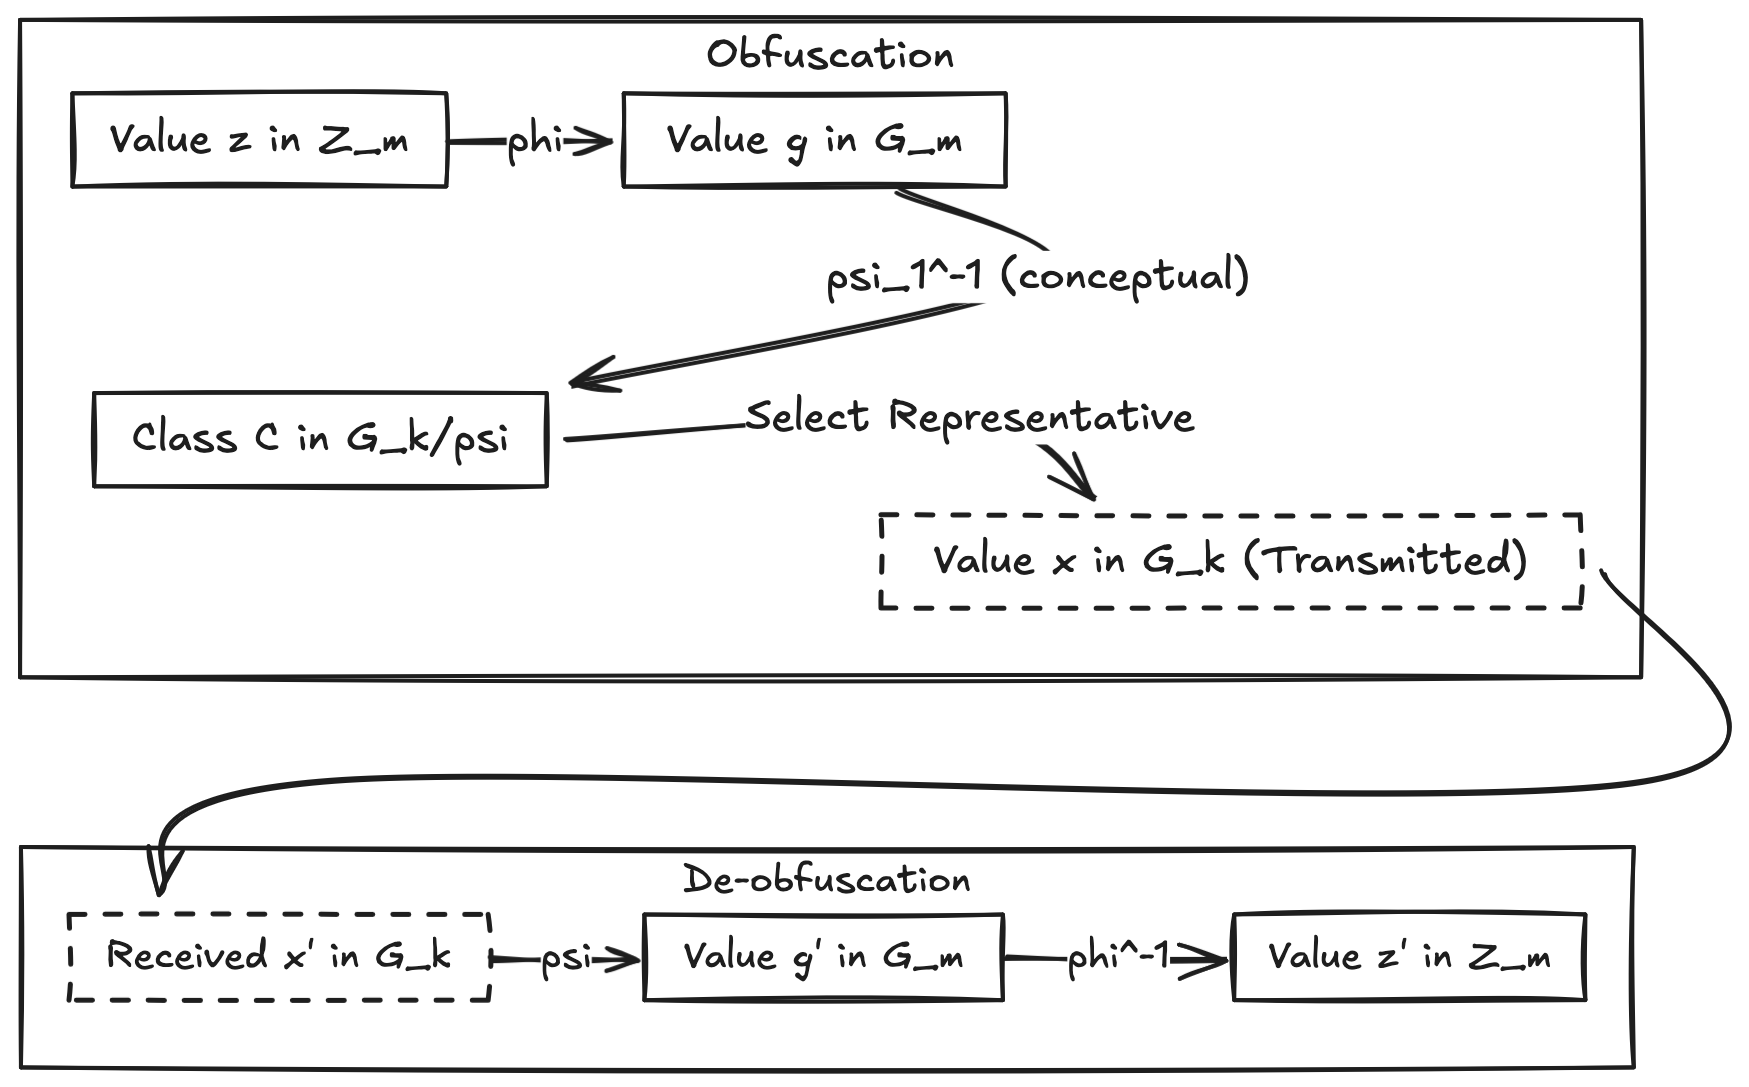
\includegraphics[width=0.9\textwidth]{pictures/De-obfuscation Data Flow Example}
    \caption{Потік даних для обфускації та де-обфускації значення.}
    \label{fig:obfuscation_flow}
\end{figure}

\section{Системи лінійних рівнянь над скінченними кільцями}
\label{sec:sle_over_rings}
Системи лінійних рівнянь (СЛР), визначені над скінченними комутативними кільцями, зокрема над кільцем лишків $Z_m$, є центральним обчислювальним механізмом запропонованої криптосистеми.
Їх властивості, критерії розв'язності та маніпуляції за допомогою матричної алгебри є фундаментальними як для процесу шифрування, так і для дешифрування.
У цьому підрозділі розширюється введення, подане у~\ref{sec:sle_theory}, зосереджуючись на аспектах, що мають безпосереднє відношення до реалізації протоколу.

\subsection{Означення та матричне представлення}
\label{subsec:sle_definition_rings}
Система лінійних рівнянь над $Z_m$ складається з $p$ лінійних конгруенцій відносно $q$ невідомих $x_1, \ldots, x_q$, які мають вигляд:
\[
    \begin{cases}
        a_{11}x_1 + a_{12}x_2 + \cdots + a_{1q}x_q \equiv b_1 \pmod{m} \\
        a_{21}x_1 + a_{22}x_2 + \cdots + a_{2q}x_q \equiv b_2 \pmod{m} \\
        \qquad \vdots \\
        a_{p1}x_1 + a_{p2}x_2 + \cdots + a_{pq}x_q \equiv b_p \pmod{m}
    \end{cases}
\]
Усі коефіцієнти $a_{ij}$, константи $b_i$ та змінні $x_j$ належать кільцю $Z_m = \{\bar{0}, \bar{1}, \ldots, \overline{m-1}\}$.
Всі арифметичні операції (додавання, віднімання, множення) виконуються за модулем $m$.

Система компактно записується у матричній формі:
\[
    Ax \equiv b \pmod{m}
\]
де:
\begin{itemize}
    \item $A = (a_{ij})$ — матриця коефіцієнтів розмірності $p \times q$, $a_{ij} \in Z_m$;
    \item $x = (x_j)$ — стовпчиковий вектор змінних розмірності $q \times 1$;
    \item $b = (b_i)$ — стовпчиковий вектор констант розмірності $p \times 1$.
\end{itemize}
У контексті криптосистеми кількість рівнянь $p$ зазвичай відповідає розміру блоку відкритого тексту, а кількість змінних $q$ обирається так, що $q \geq p$.

\subsection{Критерії розв'язності та структура розв'язків}
\label{subsec:sle_solvability_rings}
Вимогою до криптосистеми є побудова початкової СЛР $l(x) = Ax$ так, щоб конгруенція $Ax \equiv b \pmod{m}$ мала хоча б один розв'язок $\bar{x}$ для \emph{будь-якого} вектора $b \in Z_m^p$.
Критерії розв'язності СЛР над $Z_m$ є складнішими, ніж над полями, особливо при складеному $m$, через наявність дільників нуля (див.~\ref{ex:z8_ops}).
Теорія тісно пов'язана з лінійними діофантовими рівняннями (див.~\ref{subsec:diophantine}).

Достатні умови розв'язності для всіх $b$ стосуються структури матриці $A$:
\begin{enumerate}
    \item \textbf{Лінійна незалежність рядків:} Рядки матриці $A$ повинні бути лінійно незалежними за модулем $m$, тобто жоден рядок не виражається через інші з коефіцієнтами з $Z_m$, окрім тривіального випадку.
    \item \textbf{Існування оберненої підматриці:} У $A$ має існувати підматриця розмірності $p \times p$ (наприклад, стовпці з номерами $i_1, \ldots, i_p$), детермінант якої $\det(A_1)$ є дільником одиниці у $Z_m$, тобто $\gcd(\det(A_1), m) = 1$.
\end{enumerate}
Якщо ці умови виконуються, розв'язність для будь-якого $b$ гарантовано.
Оберненість $A_1$ (через $\det(A_1)$ — дільник одиниці) забезпечує існування єдиного розв'язку для квадратної підсистеми $A_1 u \equiv b \pmod{m}$, де $u$ — відповідні змінні.
Загальний розв'язок початкової системи $Ax \equiv b \pmod{m}$ будується так: координати $x_{i_j}$ прирівнюються до компонент $u$, решта — до нуля.

Варто зазначити, що при $q > p$ розв'язок $\bar{x}$ не єдиний; множина всіх розв'язків утворює афінний підпростір $Z_m^q$, що складається з одного часткового розв'язку та всіх розв'язків відповідної однорідної системи $Ax \equiv 0 \pmod{m}$.
Для шифрування достатньо знайти \emph{будь-який} розв'язок $\bar{x}$.

\subsection{Однорідні системи}
\label{subsec:sle_homogeneous}
Система $Ax \equiv b \pmod{m}$ називається \emph{однорідною}, якщо $b = 0$, тобто $Ax \equiv 0 \pmod{m}$.
Розв'язки однорідної системи (яка завжди має тривіальний розв'язок $x \equiv 0$) описують структуру множини розв'язків відповідної неоднорідної системи (будь-які два розв'язки $Ax \equiv b$ відрізняються на розв'язок $Ax \equiv 0$).

Існування нетривіальних розв'язків ($x \not\equiv 0$) залежить від властивостей $A$ та $m$.
Наприклад, для квадратної матриці ($p=q$) нетривіальні розв'язки існують тоді і тільки тоді, коли $\det(A)$ дорівнює нулю або є дільником нуля у $Z_m$.

Однорідні системи використовуються для перевірки лінійної незалежності рядків матриці коефіцієнтів $A$ у початковій системі $l(x)=Ax$.
Рядки $A$ лінійно незалежні за модулем $m$ тоді і тільки тоді, коли єдиним розв'язком транспонованої однорідної системи $A^T y \equiv 0 \pmod{m}$ є тривіальний розв'язок $y \equiv 0$.
Перевірка цієї умови є необхідним кроком при побудові допустимої матриці $A$ для криптосистеми.

\subsection{Матричні операції у $Z_m$}
\label{subsec:matrix_ops_zm}
Всі обчислення з СЛР виконуються стандартними матричними операціями, адаптованими до кільця $Z_m$.
Додавання та віднімання матриць здійснюється покомпонентно за модулем $m$.
Множення матриць виконується за стандартним правилом ``рядок на стовпець'' з приведенням усіх проміжних результатів за модулем $m$.

Обернення матриць є особливо важливою операцією у протоколі.
Воно необхідне для дешифрування (Аліса обчислює $B_i^{-1}$ для секретних матриць перетворення) та, можливо, для знаходження розв'язку $\bar{x}$ при шифруванні (якщо Боб використовує обернену підматрицю $A_1$).
Квадратна матриця $M \in Z_m^{p \times p}$ є оберненою тоді і тільки тоді, коли її детермінант $\det(M)$ є дільником одиниці у $Z_m$, тобто $\gcd(\det(M), m) = 1$.
Якщо $\det(M)$ дорівнює нулю або є дільником нуля, матриця $M$ не обернена у $Z_m$.

Якщо $\det(M)$ — дільник одиниці, обернена матриця $M^{-1}$ існує і єдина.
Її можна обчислити такими методами:
\begin{itemize}
    \item \textbf{Метод прискореної матриці (ад'юнкт-метод):} $M^{-1} \equiv (\det(M))^{-1} \cdot \mathrm{adj}(M) \pmod{m}$, де $(\det(M))^{-1}$ знаходиться за допомогою розширеного алгоритму Евкліда, а $\mathrm{adj}(M)$ — ад'юнкт-матриця.
    \item \textbf{Метод Гаусса:} Модифікований метод Гаусса застосовується до $Z_m$, причому ділення на ведучий елемент замінюється множенням на його обернений у $Z_m$.
    Якщо ведучий елемент — дільник нуля або нуль, стандартний алгоритм не застосовується і потребує модифікацій (наприклад, використання нормальної форми Сміта).
\end{itemize}
З огляду на потенційні складнощі матричних операцій, особливо обернення, у $Z_m$ при складеному $m$, доцільно використовувати ізоморфізм $\varphi: G_m \to Z_m$.
Відображуючи елементи матриць з $G_m$ у $Z_m$, всі обчислення виконуються у стандартному кільці $Z_m$ із застосуванням ефективних алгоритмів (наприклад, розширеного алгоритму Евкліда для знаходження обернених).
Отримані результати за потреби повертаються у $G_m$ через $\varphi$.
Такий підхід суттєво підвищує ефективність обчислень і спрощує реалізацію.


\section{Основний криптографічний механізм}
\label{sec:core_mechanism}
Після викладення необхідних відомостей про скінченні кільця, відображення та системи лінійних рівнянь над цими кільцями, синтезуємо ці елементи для опису основного криптографічного механізму запропонованого протоколу.
Цей механізм поєднує базову лінійну систему $l(x)$ та секретне афінне перетворення $L(x)$, а також обфускацію за допомогою ізоморфізмів і сюр'єкцій кілець для забезпечення стійкого шифрування та дешифрування.
У цьому підрозділі викладаються фундаментальні принципи цих операцій, а конкретні інтерактивні кроки між Алісою і Бобом розглядаються у Розділі~3.

\subsection{Шифрування через перетворення та обчислення СЛР}
\label{subsec:encryption_mechanism}
Основна ідея шифрування полягає у кодуванні блоку відкритого тексту $v$, представленого вектором у $Z_m^p$, за допомогою двох пов'язаних систем лінійних рівнянь $l(x)$ та $L(x)$, обчислених у спеціально вибраних точках.
Процес складається з кількох концептуальних етапів:

\begin{enumerate}
    \item \textbf{Визначення базової системи ($l(x)$):} Початково визначається базова лінійна система $l(x) = Ax$, де $A$ — матриця розмірності $p \times q$ з елементами у $G_m$ (або її еквівалент $\hat{A}$ у $Z_m$).
    Як зазначено у~\ref{subsec:sle_solvability_rings}, матриця $A$ має бути побудована так, щоб система $Ax \equiv b \pmod{m}$ була розв'язною для будь-якого вектора $b \in G_m^p$.
    Це передбачає лінійну незалежність рядків $A$ та існування оберненої підматриці розмірності $p \times p$.

    \item \textbf{Секретне афінне перетворення ($l(x) \to L(x)$):} Далі застосовується послідовність секретних афінних перетворень до базової системи $l(x)$:
    \[
        L(x) = B_r(B_{r-1}(\ldots B_2(B_1(l(x)+a_1)+a_2)\ldots + a_{r-1})+a_r)+a_{r+1}
    \]
    Тут $B_1, \ldots, B_r$ — секретні обернені матриці розмірності $p \times p$ у $G_m$, а $a_1, \ldots, a_{r+1}$ — секретні вектори розмірності $p \times 1$.
    Позначимо $D = B_r B_{r-1} \ldots B_1$ — загальна лінійна частина перетворення (також обернена).
    В результаті $L(x)$ має загальний афінний вигляд $L(x) = Bx + a$, де $B$ та $a$ залежать від $A$, $B_i$ та $a_j$.
    Послідовність $(B_i, a_j)$ є секретною.
    Всі обчислення виконуються у $G_m$ або, еквівалентно, у $Z_m$ через ізоморфізм $\varphi$.

    \item \textbf{Обчислення шифротексту:} Для шифрування конкретного блоку $v \in Z_m^p$ сторона, що шифрує (Боб), виконує такі дії, працюючи з представленнями у $Z_m$:
    \begin{itemize}
        \item \textbf{Знаходження розв'язку для відкритого тексту ($\bar{x}$):} Боб розв'язує базову систему для заданого $v$, знаходячи вектор $\bar{x} \in Z_m^q$ такий, що $\hat{l}(\bar{x}) = \hat{A}\bar{x} \equiv v \pmod{m}$.
        Оскільки $q \geq p$ і $A$ побудовано відповідно, розв'язок існує.
        Якщо розв'язків декілька, обирається будь-який.
        \item \textbf{Вибір випадкового вектора ($\bar{a}$):} Боб генерує новий випадковий вектор $\bar{a} \in Z_m^q$, незалежно для кожного блоку.
        \item \textbf{Обчислення компонент шифротексту ($d, d_1$):} Боб обчислює два вектори у $Z_m^p$:
        \begin{itemize}
            \item $d = \hat{l}(\bar{a}) = \hat{A}\bar{a} \pmod{m}$ — результат застосування базового лінійного відображення до випадкового вектора.
            \item $d_1 = \hat{L}(\bar{x} + \bar{a}) = \hat{B}(\bar{x} + \bar{a}) + \hat{a} \pmod{m}$ — результат застосування афінного перетворення до суми розв'язку та випадкового вектора.
        \end{itemize}
    \end{itemize}

    \item \textbf{Представлення та передача шифротексту:} Пара векторів $(d, d_1)$ є основною криптографічною інформацією, що представляє зашифрований блок $v$.
    Перед передачею ці вектори (у $Z_m$) обфускуються за допомогою відображень кілець: спочатку відображаються у $G_m$ через $\varphi$, далі — через бієкцію (наприклад, $\psi_1: G_k/\psi \to G_m$) кожна компонента відображається у відповідний клас фактор-множини $G_k/\psi$, після чого з кожного класу вибирається представник у $G_k$ для формування переданих векторів $(\bar{d}, \bar{d}_1)$.
    Така багаторівнева обфускація приховує справжні значення $d$ та $d_1$.
\end{enumerate}

На рисунку~\ref{fig:encryption_logic} наведено концептуальну схему процесу шифрування.
\begin{figure}[ht]
    \centering
    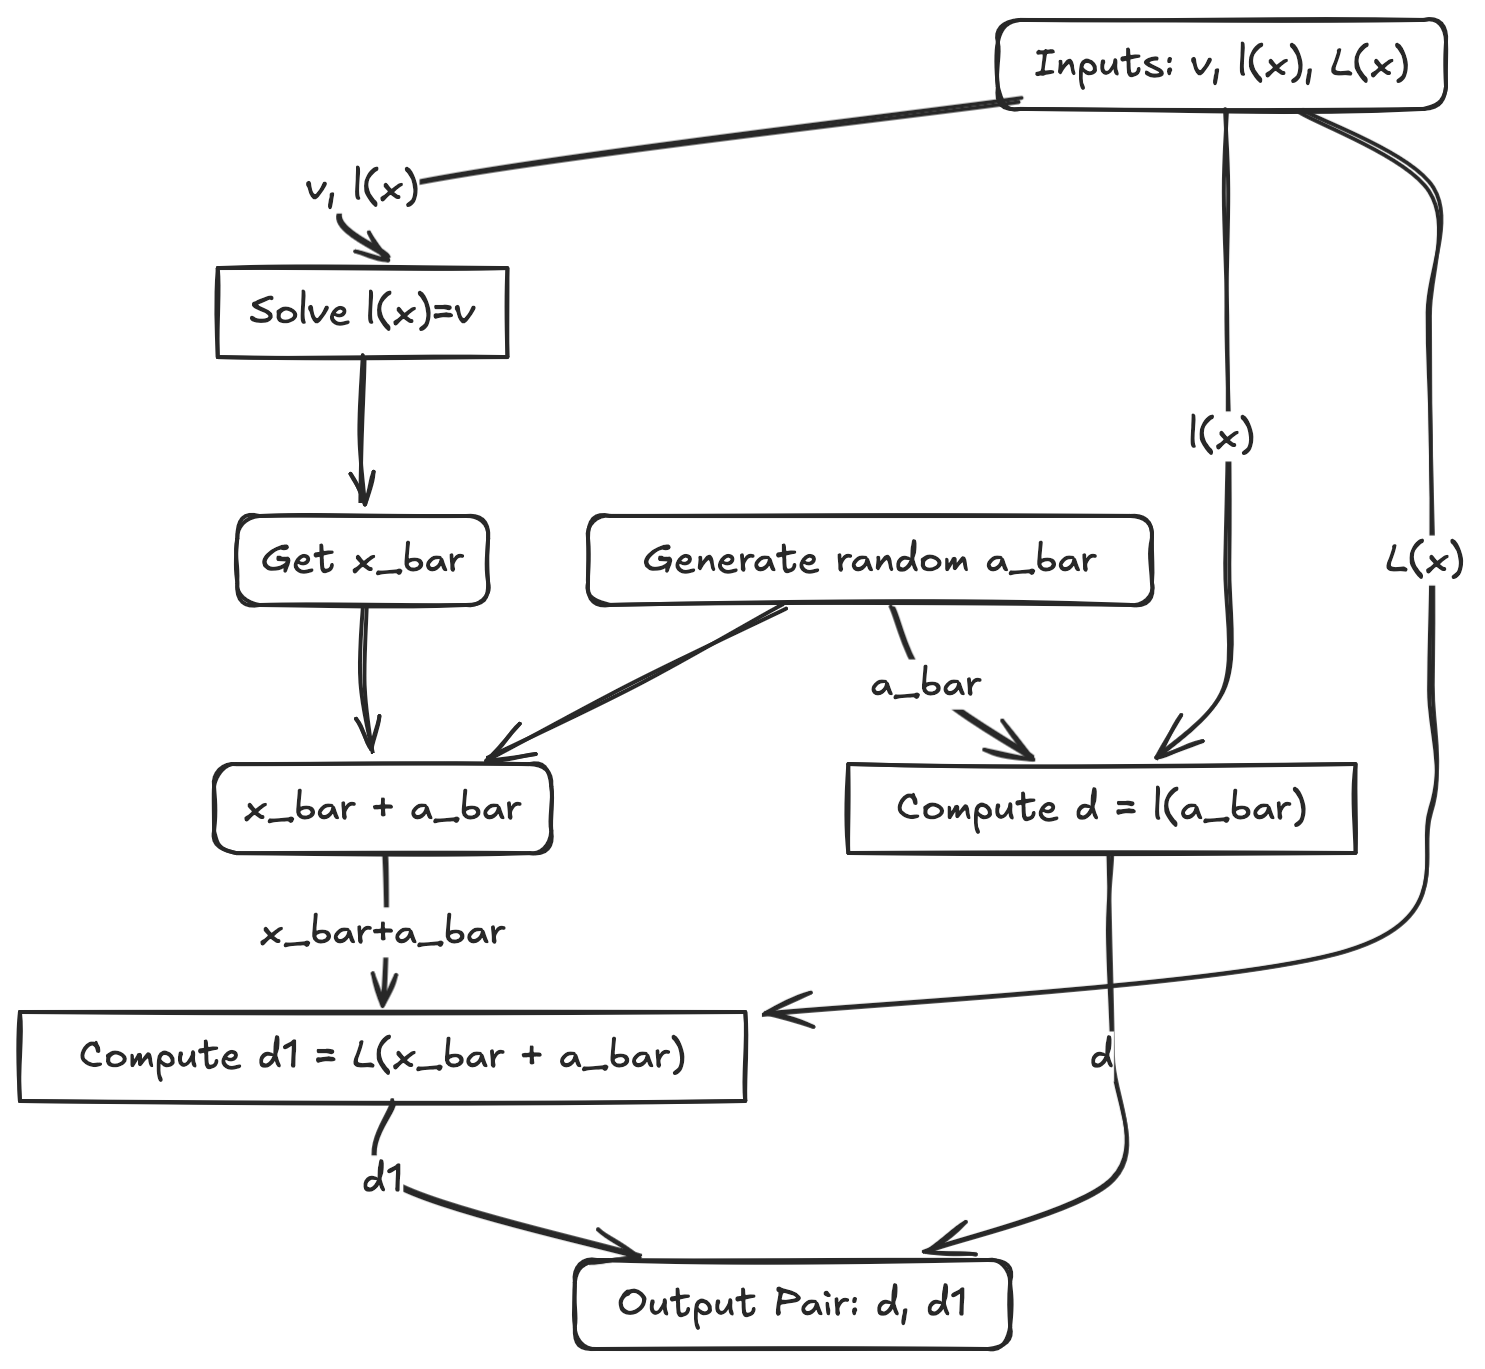
\includegraphics[width=0.5\textheight,keepaspectratio]{pictures/Encryption Core Logic Conceptual Diagram}
    \caption{Концептуальна схема процесу шифрування.}
    \label{fig:encryption_logic}
\end{figure}

\subsection{Дешифрування через зворотні перетворення}
\label{subsec:decryption_mechanism}
Дешифрування виконує сторона (Аліса), яка знає секретні компоненти: відображення ($\varphi, \psi_1$ тощо) та параметри афінного перетворення ($B_i, a_j$).
Процес полягає у зворотному відтворенні кроків шифрування для відновлення відкритого тексту $v$.

\begin{enumerate}
    \item \textbf{Відновлення основних компонент шифротексту ($d, d_1$):} Аліса отримує обфусковану пару $(\bar{d}, \bar{d}_1)$ з елементів $G_k$, застосовує зворотні відображення для отримання векторів $d, d_1$ у $Z_m$.
    Це включає використання зворотної бієкції (наприклад, $\psi_1^{-1}$) та зворотного ізоморфізму $\varphi^{-1}$.

    \item \textbf{Обчислення обернених перетворень:} Аліса обчислює обернені до секретних матриць $B_i$, переводячи їх у $Z_m$ через $\varphi^{-1}$ та знаходячи обернені $\hat{B}_i^{-1}$ у $Z_m$.
    Оскільки $\det(\hat{B}_i)$ — дільник одиниці, обернення можливе (див.~\ref{subsec:matrix_ops_zm}).
    Позначимо $D = B_r \ldots B_1$, тоді $\hat{D}^{-1} = \hat{B}_1^{-1} \ldots \hat{B}_r^{-1}$.

    \item \textbf{Зворотне афінне перетворення:} Аліса, знаючи $\hat{B}_i^{-1}$ та $\hat{a}_j = \varphi^{-1}(a_j)$, алгебраїчно відновлює $\hat{l}(\bar{x} + \bar{a}) + \hat{a}_1$ із $d_1$.
    Якщо $L(y) = D(l(y) + a_1) + c$, то
    \[
        \hat{D}^{-1}(d_1 - \hat{c}) = \hat{l}(\bar{x} + \bar{a}) + \hat{a}_1
    \]
    де $\hat{c}$ — накопичена константа, що залежить від $\hat{a}_2, \ldots, \hat{a}_{r+1}$ та $\hat{B}_i$.

    \item \textbf{Виділення відкритого тексту ($v$):} Аліса використовує $d = \hat{l}(\bar{a})$ та $\hat{a}_1$ для остаточного обчислення:
    \[
        (\hat{l}(\bar{x} + \bar{a}) + \hat{a}_1) - (\hat{l}(\bar{a}) + \hat{a}_1) = \hat{l}(\bar{x})
    \]
    Оскільки $\hat{l}(x)$ — лінійне відображення, $\hat{l}(\bar{x}) = v$, тобто відновлюється початковий блок відкритого тексту.
    Коректність цього процесу випливає з властивостей афінних перетворень та лінійності $l(x)$.
\end{enumerate}

На рисунку~\ref{fig:decryption_logic} наведено концептуальну схему процесу дешифрування.
\begin{figure}[ht]
    \centering
    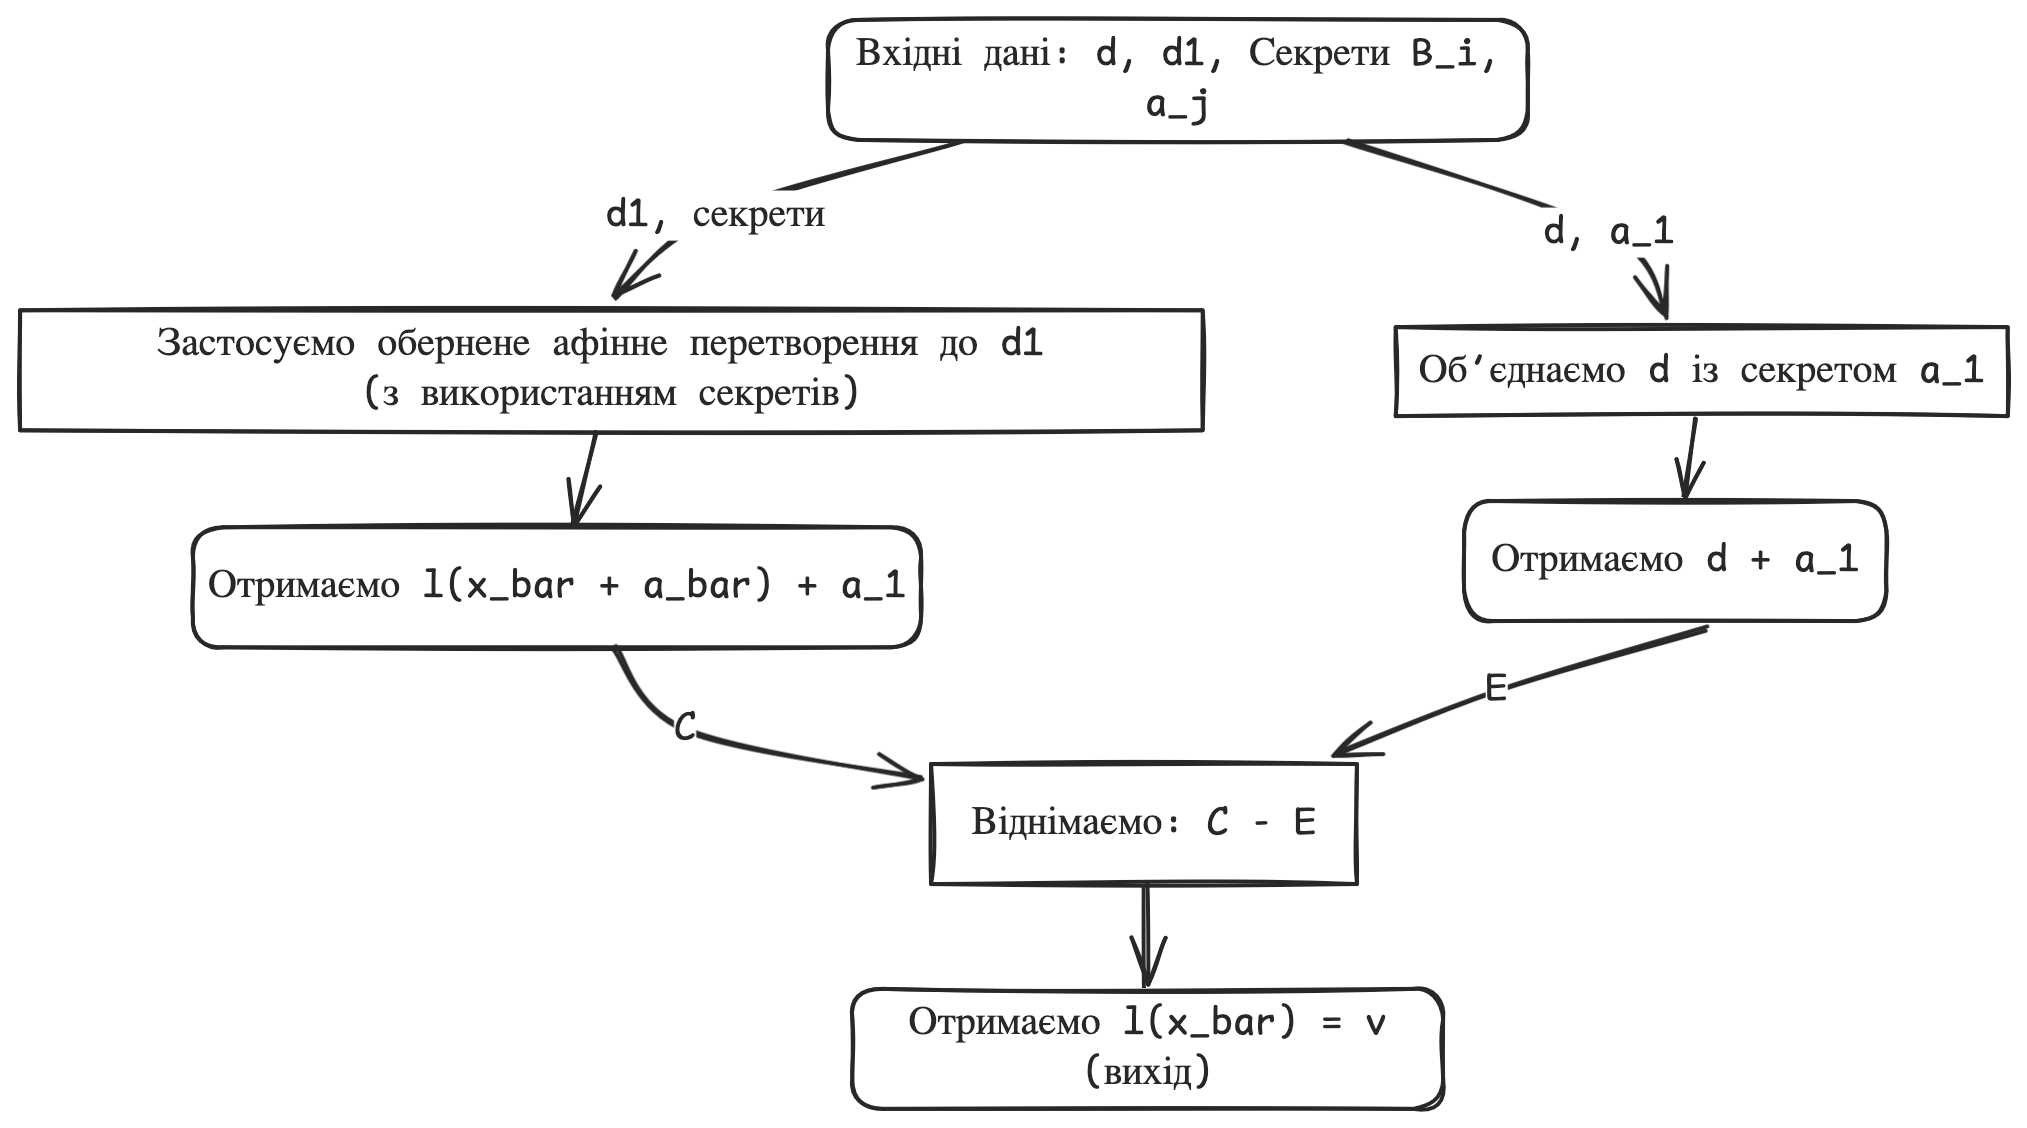
\includegraphics[width=0.9\textwidth]{pictures/Decryption Core Logic Conceptual Diagram}
    \caption{Концептуальна схема процесу дешифрування.}
    \label{fig:decryption_logic}
\end{figure}

\subsection{Роль випадковості та відображень}
\label{subsec:randomness_mappings_role}
Два компоненти є ключовими для стійкості та функціонування механізму, окрім самих перетворень СЛР: випадковий вектор $\bar{a}$ та різноманітні відображення кілець.

Випадковий вектор $\bar{a} \in Z_m^q$, що обирається Бобом для кожного блоку, відіграє роль, аналогічну до ініціалізаційного вектора у класичних симетричних шифрах, але інтегрований у схему інакше.
Його основна функція — забезпечення ймовірнісного шифрування, тобто семантичної стійкості.
Оскільки обидві компоненти шифротексту $d = \hat{l}(\bar{a})$ та $d_1 = \hat{L}(\bar{x} + \bar{a})$ залежать від $\bar{a}$, шифрування одного й того ж блоку $v$ у різний час дає статистично незалежні пари $(\bar{d}, \bar{d}_1)$.
Це унеможливлює частотний аналіз.

Відображення кілець ($\varphi, \psi, \lambda, \psi_1, \lambda_1$) виконують декілька функцій:
\begin{itemize}
    \item \textbf{Обчислювальна ефективність ($\varphi$):} Ізоморфізм $\varphi: Z_m \to G_m$ дозволяє виконувати всі складні обчислення (обернення матриць, розв'язання СЛР) у стандартному кільці $Z_m$.
    \item \textbf{Структурна обфускація ($G_m$):} Використання $G_m$ замість $Z_m$ приховує структуру модульної арифметики, ускладнюючи застосування класичних атак без знання ізоморфізму $\varphi$.
    \item \textbf{Обфускація представлення ($\psi, \lambda, \psi_1, \lambda_1$):} Сюр'єкції та бієкції фактор-множин дозволяють представляти значення з $Z_m$ або $G_m$ зовнішньо як елементи з більшого кільця $G_k$, приховуючи справжню структуру та значення $d, d_1$.
    Для атакуючого, що спостерігає $\bar{d}, \bar{d}_1$ у $G_k$, відновлення $d, d_1$ у $Z_m$ вимагає знання секретних відображень.
\end{itemize}
У сукупності ці відображення створюють багаторівневий захист, що вимагає від атакуючого розкриття кількох структурних секретів, окрім вирішення основної алгебраїчної задачі для перетворених СЛР.


\section{Архітектура системи та генерація компонентів}
\label{sec:architecture_generation}
Після детального розгляду основних алгебраїчних структур, відображень і криптографічного механізму, переходимо до загальної архітектури системи та процесу генерації її ключових компонентів.
Практична реалізація криптосистеми ґрунтується на детермінованому методі побудови необхідних кілець і відображень із набору спільних секретних параметрів, що гарантує узгодженість алгебраїчного середовища для обох абонентів, навіть якщо воно є обфускованим.

\subsection{Схематичний огляд системи}
\label{subsec:system_diagram}
Концептуальна архітектура криптосистеми зображена на рис.~\ref{fig:schema}.

\begin{figure}[ht]
  \centering
  \begin{tikzpicture}[node distance=1.5cm and 2.5cm, >=latex]
    % Define Nodes
    \node (Zm)                  {\(Z_m\)};
    \node (Gm_top) [right=of Zm, yshift=1.5cm] {\(G_m\)};
    \node (Gm_bot) [right=of Zm, yshift=-1.5cm]{\(G_m\)};
    \node (Gk)     [right=of Gm_top, xshift=1cm, yshift=-1.5cm] {\(G_k\)};
    \node (Gk_psi) [above=of Gk] {\(G_k/\psi\)};
    \node (Gk_lam) [below=of Gk] {\(G_k/\lambda\)};

    % Z_m <-> G_m (top)
    \draw[->] (Zm) -- node[above, sloped] {\(\varphi\)} (Gm_top);
    \draw[->] (Gm_top) -- node[below, sloped] {} (Zm);

    % Z_m <-> G_m (bottom)
    \draw[->] (Zm) -- node[below, sloped] {\(\varphi\)} (Gm_bot);
    \draw[->] (Gm_bot) -- node[above, sloped] {} (Zm);

    % G_k -> G_m (top & bottom)
    \draw[->] (Gk) -- node[above, sloped] {\(\psi\)} (Gm_top);
    \draw[->] (Gk) -- node[below, sloped] {\(\lambda\)} (Gm_bot);

    % G_k -> G_k factor rings
    \draw[->] (Gk) -- (Gk_psi);
    \draw[->] (Gk) -- (Gk_lam);

    % Factor rings -> G_m
    \draw[->] (Gk_psi) -- node[above] {\(\psi_1\)} (Gm_top);
    \draw[->] (Gm_top) -- node[below] {} (Gk_psi);

    \draw[->] (Gk_lam) -- node[below] {\(\lambda_1\)} (Gm_bot);
    \draw[->] (Gm_bot) -- node[above] {} (Gk_lam);

  \end{tikzpicture}
  \caption{Схема системи}
  \label{fig:schema}
\end{figure}

Ця схема ілюструє взаємозв'язки та можливі потоки даних між різними алгебраїчними компонентами:
\begin{itemize}
    \item \textbf{$Z_m$}: Стандартне кільце лишків за модулем $m$. Основна роль — домен для ефективних обчислень, зокрема для матричних операцій (обернення, розв'язання СЛР).
    \item \textbf{$G_m$}: Робоче кільце, ізоморфне $Z_m$ через $\varphi$. У цьому кільці концептуально визначаються та маніпулюються системи $l(x)$ і $L(x)$. Використання $G_m$ забезпечує структурну обфускацію, оскільки його представлення залежить від секретного визначального рядка.
    \item \textbf{$G_k$}: Більше кільце, ізоморфне $Z_k$ ($k=lm$), використовується переважно як джерело для обфускованих представлень значень, що походять з $G_m$ або $Z_m$.
    \item \textbf{$\psi, \lambda$}: Дві різні сюр'єктивні гомоморфізми кілець, що відображають елементи з $G_k$ у робоче кільце $G_m$. Вони визначають зв'язок між простором представлення $G_k$ та обчислювальним простором $G_m$.
    \item \textbf{$G_k/\psi, G_k/\lambda$}: Фактор-множини (класи суміжності), породжені сюр'єкціями $\psi$ та $\lambda$. Кожен елемент у $G_k/\psi$ (або $G_k/\lambda$) — це підмножина $G_k$, що містить усі елементи, які відображаються у той самий елемент $G_m$ через $\psi$ (або $\lambda$). Ці фактор-множини слугують проміжними структурами для зовнішнього представлення даних.
    \item \textbf{$\psi_1, \lambda_1$}: Бієкції, що встановлюють взаємно однозначну відповідність між фактор-множинами $G_k/\psi$ (або $G_k/\lambda$) та кільцем $G_m$. Вони забезпечують механізм переходу між елементом у $G_m$ та відповідним класом прообразу, дозволяючи вибирати представників із $G_k$ для зовнішньої комунікації.
    \item \textbf{$\varphi$}: Ключовий ізоморфізм, що пов'язує $G_m$ та $Z_m$, забезпечуючи перехід між потенційно обфускованим робочим кільцем $G_m$ та ефективним обчислювальним кільцем $Z_m$.
\end{itemize}
Архітектура підтримує декілька шляхів представлення та обробки даних. Наприклад, у типовому варіанті протоколу: Аліса визначає $l(x)$ і $L(x)$ у $G_m$, відображає їх коефіцієнти через $\lambda_1$ у $G_k/\lambda$, публікує представників із $G_k$. Боб отримує ці дані, повертає їх через $\lambda_1^{-1}$ у $G_m$, далі через $\varphi^{-1}$ у $Z_m$ для отримання $\hat{l}(x), \hat{L}(x)$ для обчислень. Боб обчислює компоненти шифротексту $d, d_1$ у $Z_m$, відображає їх через $\varphi$ у $G_m$, далі через $\psi_1$ у $G_k/\psi$ і передає представників із $G_k$. Аліса виконує зворотне відображення через $\psi_1^{-1}$ та $\varphi^{-1}$ для отримання $d, d_1$ у $Z_m$ для дешифрування. Такий багаторівневий підхід із залученням кількох кілець і відображень спрямований на обфускацію обчислень і даних від зовнішніх спостерігачів.

\subsection{Генерація кілець і відображень (алгоритм GEN-G)}
\label{subsec:gen_g_algorithm}
Конкретні екземпляри ізоморфних кілець $G_k$ і $G_m$, а також ключовий ізоморфізм $\varphi: Z_m \to G_m$, не вибираються довільно, а генеруються детерміновано з набору спільних секретних параметрів за допомогою алгоритму GEN-G.

\textbf{Алгоритм GEN-G$(a,c,l,k)$:}
\begin{itemize}
    \item \textbf{Вхід:} Набір секретних цілих параметрів $(a, c, l, k)$. Тут $k$ — порядок більшого кільця $G_k$, $m$ ($k=lm$) — порядок робочого кільця $G_m$, а $a, c$ — коефіцієнти лінійної конгруентної функції $f(i) = a \cdot i + c$. Важливою умовою є $\gcd(a, k) = 1$, що гарантує, що при пробіганні $i$ по повній системі лишків за модулем $k$, значення $a \cdot i + c \pmod{k}$ також утворюють повну систему лишків, тобто перестановку.
    \item \textbf{Вихід:} Визначальний рядок $b = (b_1, b_2, \ldots, b_k)$ для кільця $G_k$, який неявно визначає його структуру та ізоморфізм із $Z_k$.
    \item \textbf{Метод:} Алгоритм складається з кількох послідовних кроків:
    \begin{enumerate}
        \item \textbf{Генерація початкового рядка:} Створюється масив $b'$ довжини $k$ за лінійною конгруентною функцією:
        \[
            \text{for } i = 0 \text{ to } k-1 \text{ do } b'[i+1] := (a \cdot i + c) \pmod{k}
        \]
        Оскільки $\gcd(a,k)=1$, масив $b'$ є перестановкою елементів $\{0, 1, \ldots, k-1\}$.
        \item \textbf{Секретне перетворення:} Початковий рядок $b'$ трансформується згідно з набором заздалегідь погоджених секретних правил, відомих лише Алісі та Бобу. Ці правила визначають послідовність перестановок або інших модифікацій масиву (наприклад, обмін сусідніх елементів, циклічні зсуви тощо). Конкретна послідовність таких перетворень є частиною секретного ключа і суттєво збільшує кількість можливих визначальних рядків. Обидва абоненти повинні застосовувати ідентичні перетворення у тій самій послідовності.
        \item \textbf{Нормалізація (фіксація 0 та 1):} Трансформований масив нормалізується: елемент зі значенням 1 розміщується на першій позиції, а елемент зі значенням 0 — на останній. Отриманий масив $b = (b_1=1, b_2, \ldots, b_{k-1}, b_k=0)$ є фінальним визначальним рядком, що повністю визначає кільце $G_k$ та ізоморфізм $g: Z_k \to G_k$. Відображення задається як $g(\bar{1}) = b_1 = 1$, $g(\bar{i}) = b_i$ для $i=2, \ldots, k-1$, $g(\bar{0}) = b_k = 0$. Ізоморфізм $\varphi: Z_m \to G_m$, необхідний для протоколу, отримується або запуском цього ж процесу з параметрами $(a, c, 1, m)$, або відповідним обмеженням/адаптацією $g$ для $G_m$.
        \item \textbf{Генерація відображення наступника (опціонально):} З фінального визначального рядка $b$ будується допоміжний масив $P[0 \ldots k-1]$, що реалізує операцію "додати одиницю" у $G_k$: $P[0] := b_1 (=1)$; $P[b_i] := b_{i+1}$ для $i=1, \ldots, k-2$; $P[b_{k-1}] := b_k (=0)$. Це відображення може використовуватись для побудови повних таблиць операцій у $G_k$, але на практиці достатньо ізоморфізму $\varphi$ для ефективних обчислень у $Z_m$.
    \end{enumerate}
\end{itemize}
Правильність алгоритму ґрунтується на тому, що лінійна конгруентна функція породжує перестановку при $\gcd(a,k)=1$ (див.~\ref{subsec:residue_rings}).
Обчислювальна складність визначається $k$ операціями множення за модулем, тобто $O(k \log^2 k)$, що є прийнятним для відносно невеликих $k$.

Важливо підкреслити, що алгоритм GEN-G генерує лише кільця $G_k, G_m$ та ізоморфізм $\varphi$.
Інші критично важливі секретні компоненти криптосистеми — конкретні сюр'єкції $\psi, \lambda$, відповідні бієкції $\psi_1, \lambda_1$, а також параметри секретних афінних перетворень $B_i, a_j$ — мають бути погоджені окремо між Алісою та Бобом через захищений канал або виведені з початкових секретів за додатковою домовленістю.
Ці додаткові компоненти завершують повну специфікацію спільного симетричного ключа.


\section{Теоретичні аспекти стійкості}
\label{sec:theoretical_security}
Стійкість запропонованої симетричної криптосистеми, як і будь-якої криптографічної схеми, ґрунтується на припущенні про обчислювальну складність певних базових математичних задач для супротивника, який має доступ лише до публічної інформації (наприклад, відкритих систем $\bar{l}(x), \bar{L}(x)$ та перехоплених шифротекстів $(\bar{d}, \bar{d}_1)$), але не володіє спільними секретними компонентами ключа.
Сила системи зумовлена поєднанням факторів, пов'язаних із комбінаторною складністю визначення секретних відображень між кільцями та труднощами зворотного відтворення секретних алгебраїчних перетворень, застосованих до систем лінійних рівнянь.

\subsection{Складність визначення ізоморфізмів та відображень}
\label{subsec:hardness_mappings}
Вагома частина стійкості системи забезпечується обфускацією, яку створюють нестандартні представлення кілець ($G_m, G_k$) та відображення між ними ($\varphi, \psi, \lambda, \psi_1, \lambda_1$).
Атакуючий, що намагається зламати систему, повинен спочатку (або паралельно) визначити ці секретні структури та відображення.

\begin{itemize}
    \item \textbf{Визначення ізоморфізму $\varphi$:} Ізоморфізм $\varphi: Z_m \to G_m$ задається визначальним рядком $b = (1, b_2, \ldots, b_{m-1}, 0)$, згенерованим алгоритмом GEN-G (див.~\ref{subsec:gen_g_algorithm}). Без знання секретних параметрів $(a, c)$ і, головне, секретних правил перетворення на відповідному кроці GEN-G, атакуючий стикається із задачею відновлення правильної перестановки $b_2, \ldots, b_{m-1}$ елементів $\{2, 3, \ldots, m-1\}$. Кількість таких перестановок становить $(m-2)!$. Додатково, секретні перетворення означають, що отриманий визначальний рядок може не відповідати жодній послідовності, згенерованій лише початковою лінійною конгруентною функцією. Це робить повний перебір ізоморфізмів обчислювально нездійсненним, оскільки простір пошуку зростає факторіально з $m$.
    \item \textbf{Визначення сюр'єкцій та фактор-множин ($\psi, \lambda, \psi_1, \lambda_1$):} Атакуючий також має визначити конкретні сюр'єктивні гомоморфізми $\psi, \lambda: G_k \to G_m$ та відповідні бієкції $\psi_1, \lambda_1$, що пов'язують фактор-множини $G_k/\psi, G_k/\lambda$ з $G_m$. Знаходження конкретного гомоморфізму між двома кільцями — загалом складна задача. У цьому випадку атакуючий повинен визначити правильне відображення з $G_k$ (структура якого вже прихована власним ізоморфізмом $\varphi_k$) на $G_m$ (структура якого прихована $\varphi$). Кількість можливих сюр'єктивних гомоморфізмів залежить від структури кілець та їх ідеалів. Для розбиття $k$ елементів $G_k$ на $m$ непорожніх підмножин (прообрази або класи суміжності), кожна з яких відображається у унікальний елемент $G_m$, кількість варіантів оцінюється як $O(k! / (m! (l!)^m))$, де $l = k/m$. Для $k=50, m=25, l=2$ це $\frac{50!}{25!(2!)^{25}}$, що є надзвичайно великим числом.
\end{itemize}

У сукупності ці фактори дають нижню межу складності повного перебору для відновлення всіх відображень навіть для відносно невеликих порядків кілець. Ця комбінаторна складність є основною лінією захисту.

\subsection{Стійкість, що випливає з перетворень СЛР}
\label{subsec:security_sle_transform}
Окрім складності визначення структур кілець і відображень, додатковий рівень стійкості забезпечується секретним афінним перетворенням, застосованим до систем лінійних рівнянь.
Розглянемо сильну модель атакуючого, який, припустимо, зумів визначити кільця $G_m, G_k$ та всі відповідні відображення ($\varphi, \psi, \lambda, \psi_1, \lambda_1$).
Тобто атакуючий може перевести відкриті системи $\bar{l}(x), \bar{L}(x)$ та перехоплені шифротексти $(\bar{d}, \bar{d}_1)$ у їх еквіваленти $\hat{l}(x), \hat{L}(x)$ та $(d, d_1)$ у стандартному кільці $Z_m$.
Навіть у такому випадку залишаються суттєві перешкоди:

\begin{itemize}
    \item \textbf{Секретність афінного перетворення:} Ядро механізму шифрування — це перетворення $l(x) \to L(x)$, визначене послідовністю секретних обернених матриць $B_i$ та секретних векторів $a_j$.
    Дешифрування вимагає знання цих $B_i$ та $a_j$ для зворотного відтворення, зокрема обчислення та застосування обернених матриць $B_i^{-1}$ і віднімання впливу векторів $a_j$ у правильному порядку (див.~\ref{subsec:decryption_mechanism}). Атакуючий, який знає лише кінцеву афінну систему $\hat{L}(x)$ (і базову $\hat{l}(x)$), але не проміжні кроки ($B_i, a_j$), не може виконати це зворотне перетворення. Задача декомпозиції афінного відображення $\hat{L}(x)$ для відновлення $\hat{l}(x)$ без знання $B_i$ та $a_j$ є обчислювально складною, оскільки існує багато різних послідовностей перетворень, що можуть призвести до одного й того ж $\hat{L}(x)$.
    \item \textbf{Обфускація випадковістю ($\bar{a}$):} Випадковий вектор $\bar{a}$, що обирається для кожного шифрування, ускладнює задачу для атакуючого.
    Він спостерігає $d = \hat{l}(\bar{a})$ та $d_1 = \hat{L}(\bar{x} + \bar{a})$, де $v = \hat{l}(\bar{x})$ — невідомий відкритий текст, $\bar{x}$ — невідомий розв'язок, а $\bar{a}$ — невідомий випадковий вектор.
    Навіть якщо $\hat{l}$ і $\hat{L}$ (тобто $\hat{A}, \hat{B}, \hat{a}$) відомі, атакуючий має лише дві відомі величини ($d, d_1$), пов'язані рівняннями з двома невідомими векторами ($\bar{x}, \bar{a}$) та невідомим $v$.
    Випадковий вектор $\bar{a}$ фактично виконує роль одноразової маски, що приховує зв'язок між $\bar{x}$ (а отже, і $v$) та шифротекстом. Без знання $\bar{a}$ атакуючий не може ізолювати компоненти, пов'язані лише з $\bar{x}$ чи $v$.
\end{itemize}
Отже, навіть якщо структурна обфускація через відображення кілець буде подолана, стійкість системи спирається на складність алгебраїчного зворотного відтворення секретного афінного перетворення $L(x)$ за відомими $l(x)$ і $L(x)$, особливо
